\section{Instrument Signature Removal}
\label{sec:isr}

Raw images from charge-coupled devices (CCDs) contain instrumental effects, such as dark currents, clocking artifacts or crosstalk between neighboring amplifiers, that can be removed in the data processing.
In the Rubin pipeline, this step is called Instrument Signature Removal (ISR) and is the first processing applied to a raw CCD exposure.
The package performing the ISR on an exposure, called \texttt{ip\_isr}, is detailed below in Sec. \ref{sec:ip_isr}: it is a critical package for Data Release Pipeline (DRP) used to process LSST images and requires calibration products produced and verified by \texttt{cp\_pipe} and \texttt{cp\_verify} respectively as described in Sec. \ref{sec:calib_pipe}.
In Sec. \ref{sec:isr:ampoffset}, we specifically describe the correction of amplifier offset in more details.

We note that we focus here on our approach to perform ISR on data from LSST cameras only (LSSTCam, ComCam and LATISS), although we also provide calibration pipelines for other cameras such as DECam and HSC (using a different ISR approach).

\subsection{ISR package}
\label{sec:ip_isr}

Exposures from LSST cameras are affected by instrumental effects, ranging from well-known CCD effects like dark currents or biases to effects more recently characterized like tree-rings (see \cite{park_properties_2017,park_tree_2020,esteves_photometry_2023} for more details on tree rings in LSSTCam) or the Brighter-Fatter effect as discussed in \cite{broughton_2023}. Correcting for these effects requires specific calibrations, which we refer to as calibration products. In LSST cameras, calibration products typically are a combined bias, a combined dark, a Photon Transfer Curve (PTC), a crosstalk matrix, a list of defects and a look-up table of non-linearity parameters.
The meaning of these calibration products and the details on the Rubin Observatory's ISR and calibration approach can be found in \url{https://sitcomtn-086.lsst.io/v/SITCOM-949/index.html}.

The \texttt{ip\_isr} package\footnote{\url{https://github.com/lsst/ip_isr}} contains the codes needed to remove instrument signatures in exposures from LSST cameras and to produce calibration products.
To inform our ISR approach, we first designed a model of the instrument, displayed in Fig. \ref{fig:isr_model}, based on our knowledge of the hardware and electronics. This model states the order in which the different known instrumental effects happen, from a photon hitting the CCD to the output ADC unit (ADU) signal.
In turn, \texttt{isrTaskLSST} in \texttt{ip\_isr} sequentially applies correction of these effects, typically by calling other \texttt{Tasks} (\textit{e.g.} overscan, crosstalk, etc.) also implemented in \texttt{ip\_isr}.


\begin{figure}[h!]
    \centering
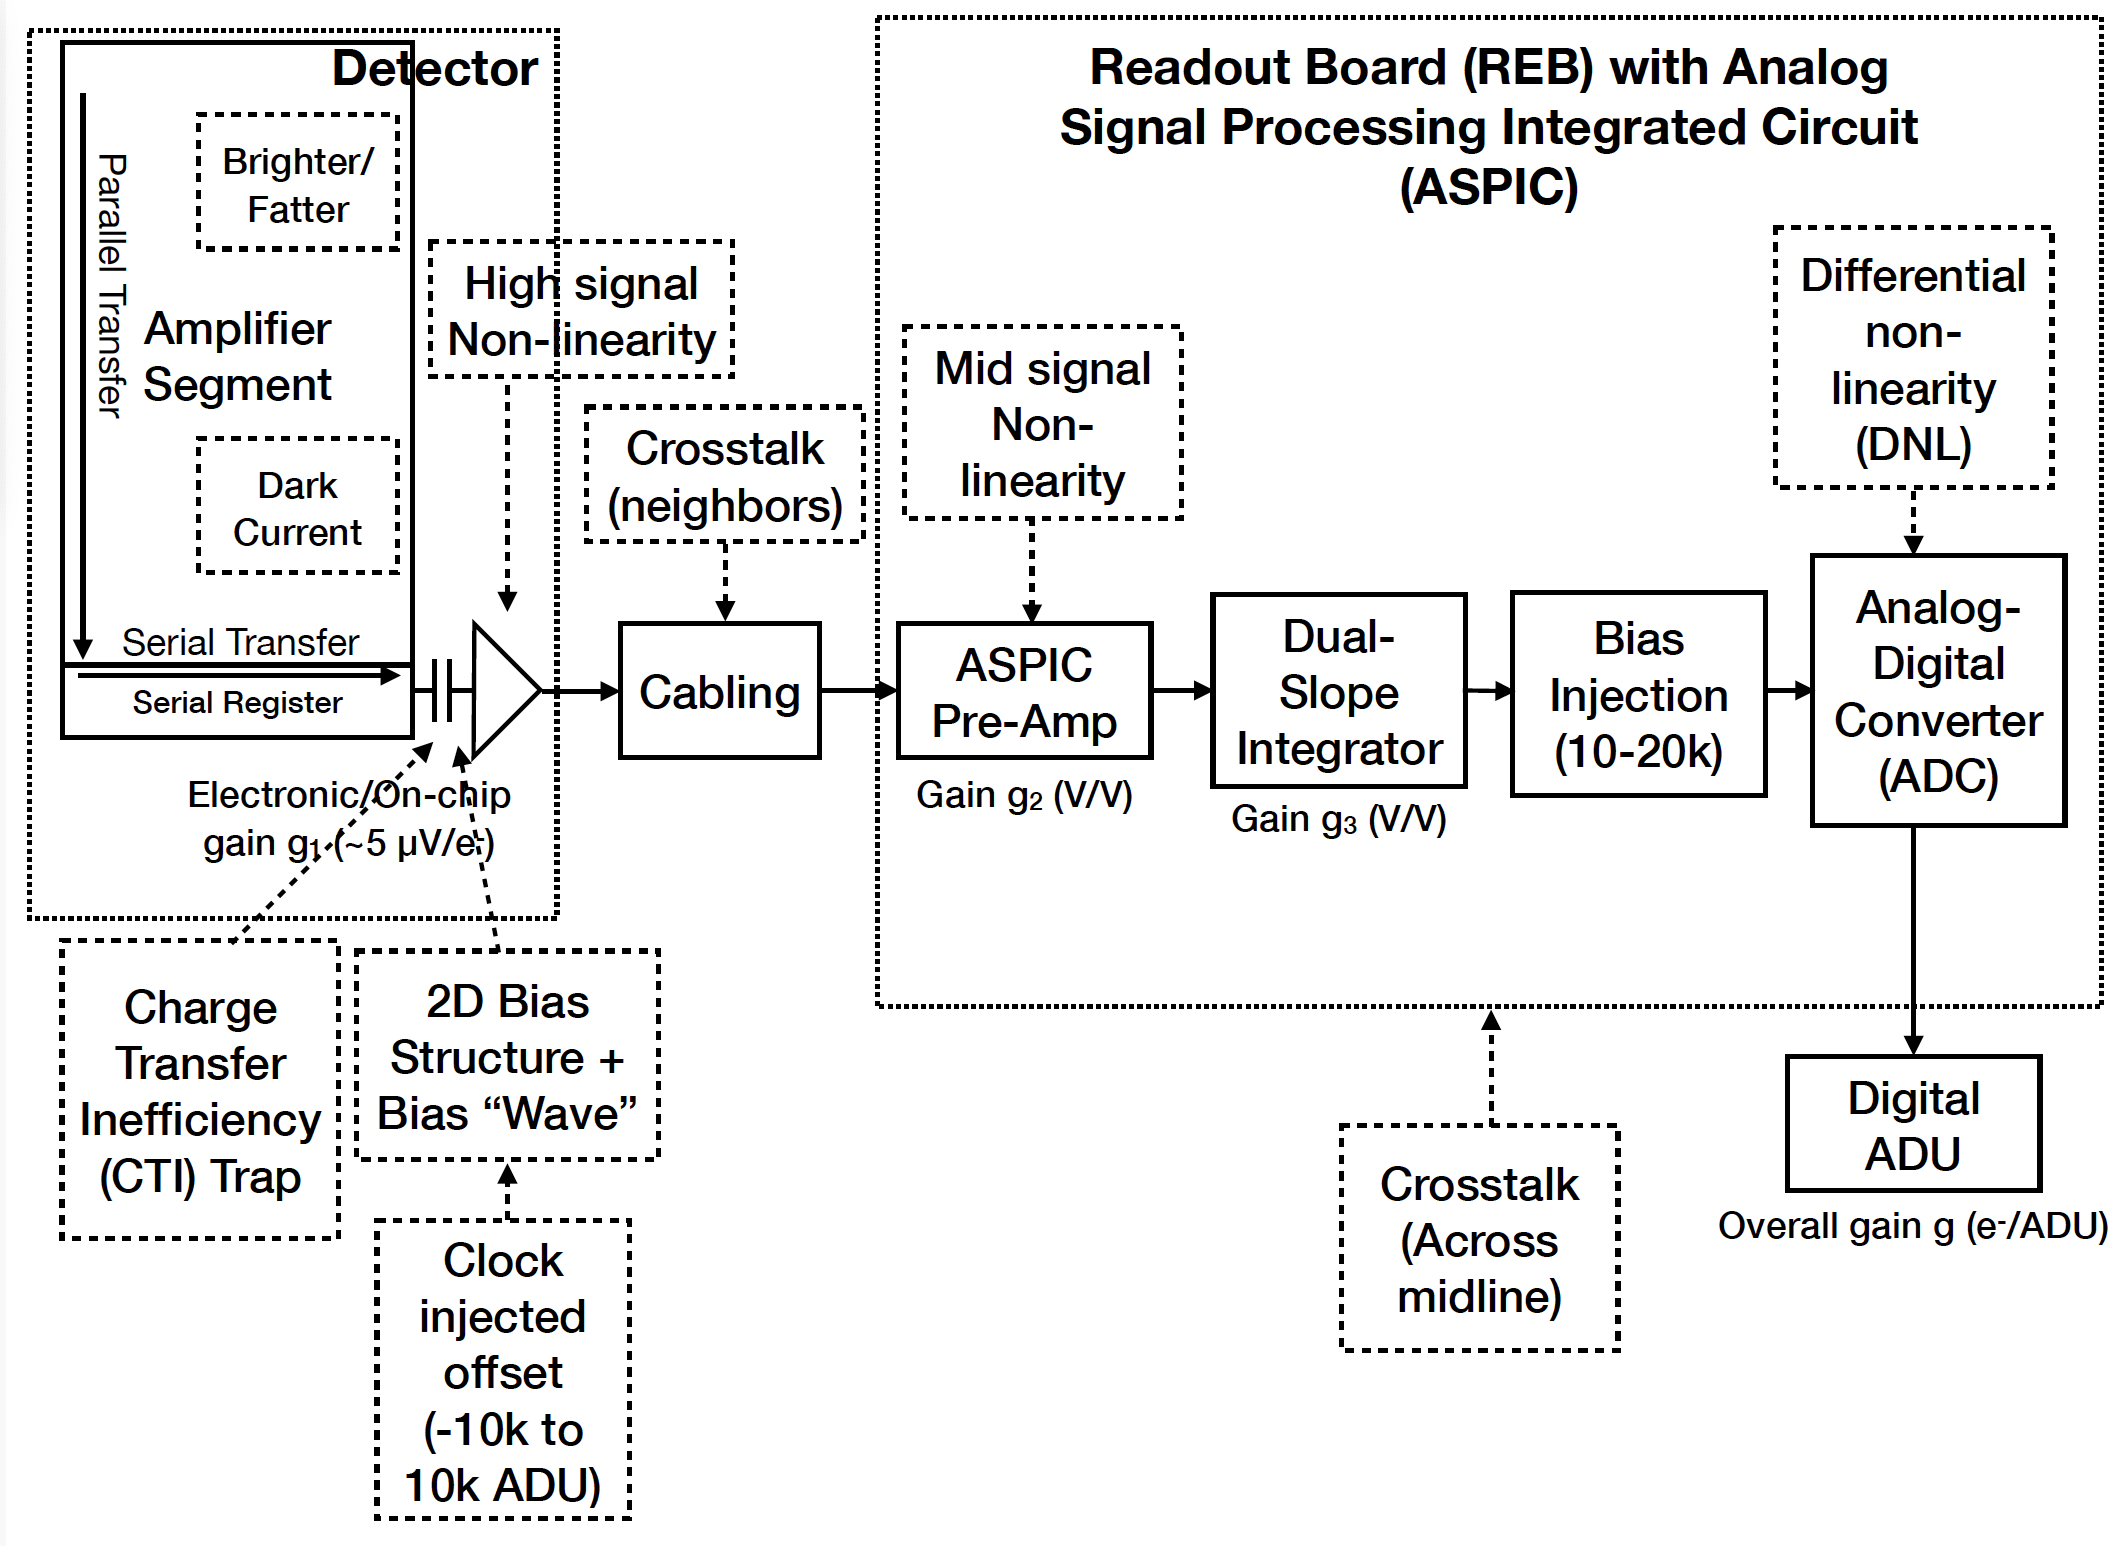
\includegraphics[scale=0.25]{isr_plots/instrumentmodel_isr.png}
    \caption{Schematic of the instrument model for detector effects in LSST cameras which \texttt{isrTaskLSST} is based on at the time of publication. Diagram made by Eli Rykoff, more details about the model can be found in \url{https://sitcomtn-086.lsst.io/v/SITCOM-949/index.html}.}
    \label{fig:isr_model}
\end{figure}


Overall, \texttt{isrTaskLSST} takes a \texttt{raw} CCD exposure, and calibration products if available, and outputs a \texttt{Struct} containing the input exposure, the \texttt{postISRCCD} output exposure as well as its binned version for easier display, the exposure before interpolation and statistics on the output exposure.
\texttt{IsrTaskLSSTConfig} defines the configurations used in this \texttt{Task}, they are set by default to their expected value to perform ISR on a typical LSSTCam exposure. Configurations starting with \texttt{do} will typically correspond to an ISR step, they are turned on or off in the pipelines when producing the different calibration products.
We have also developed \texttt{isrMockLSST} which simulates a raw exposure and corresponding calibration products and is used to test \texttt{isrTaskLSST}.


\subsection{Amplifier Offset Correction}
\label{sec:isr:ampoffset}
The amplifier offset correction (commonly referred to as amp-offset correction, or pattern continuity correction) runs as part of the instrument signature removal (ISR) process.
This correction is designed to address systematic discontinuities in background sky levels across amplifier boundaries.
We believe that these discontinuities arise from electronic biases between adjacent amplifiers, persisting even after application of dark and flat corrections.

Drawing on the \texttt{PANSTARRS}' Pattern Continuity algorithm \citep{2020ApJS..251....4W}, our method aims to eliminate these offsets, thereby preventing problems such as background over-/under-subtraction at amplifier boundaries caused by discontinuities across the detector.

The amp-offset algorithm initially computes a robust flux difference measure between two narrow strips on opposite sides of each amplifier-amplifier interface.
Regions containing detected sources, or pixel data which have been masked for other reasons, are not considered.
These amp-interface differences are stored in an amp-offset matrix; diagonal entries represent the number of neighboring amplifiers, and off-diagonal entries encode information about the associations between amplifiers.
A complementary interface matrix encodes directional information for these associations.
Using this information, a least-squares minimization is performed to determine the optimal pedestal value to be added or subtracted to each amp which would reduce the amp-offset between that amplifier and all of its neighboring amplifiers.
This method is generalized to support 2D amplifier geometries within a detector, as with LSSTCam, incorporating length-based weighting into the matrices to account for amplifiers that are not square.

\subsection{Calibration pipelines}
\label{sec:calib_pipe}

The pipelines to build calibration products (\texttt{cp}) for the LSST cameras are defined in \texttt{cp\_pipe}\footnote{\url{https://github.com/lsst/cp\_pipe} and see documentation at \url{https://pipelines.lsst.io/modules/lsst.cp.pipe/constructing-calibrations.html}}.
They mainly set \texttt{isrTaskLSST} configurations needed for each calibration product. In some cases, they also specify whether to combine exposures (for bias or dark exposures for instance) and to bin exposures to support display.

Once calibration products are produced, they are ``verified'' using \texttt{cp\_verify} pipelines by checking they pass metrics defined in \url{https://dmtn-101.lsst.io/}. They then can be certified and used to ISR an exposure.
